% =====================================================================
% Figure: Traceability matrix for the indoor robot (excerpt)
% Matches Chapter 20, section "Traceability Matrix"
%
% Used in the book, e.g. in chapters_en/20_traceability.tex:
%
%   \begin{figure}[H]
%     \centering
%     % =====================================================================
% Figure: Traceability matrix for the indoor robot (excerpt)
% Matches Chapter 20, section "Traceability Matrix"
%
% Used in the book, e.g. in chapters_en/20_traceability.tex:
%
%   \begin{figure}[H]
%     \centering
%     % =====================================================================
% Figure: Traceability matrix for the indoor robot (excerpt)
% Matches Chapter 20, section "Traceability Matrix"
%
% Used in the book, e.g. in chapters_en/20_traceability.tex:
%
%   \begin{figure}[H]
%     \centering
%     % =====================================================================
% Figure: Traceability matrix for the indoor robot (excerpt)
% Matches Chapter 20, section "Traceability Matrix"
%
% Used in the book, e.g. in chapters_en/20_traceability.tex:
%
%   \begin{figure}[H]
%     \centering
%     \input{figures_en/fig_kap20_traceability_matrix}
%     \caption{Excerpt from a traceability matrix: each row connects
%       a requirement, through a function, system element, and ROS2
%       node, to a test case.}
%     \label{fig:kap20-traceability-matrix}
%   \end{figure}
%
% Required packages (already loaded in main_en.tex): tikz
% Required TikZ libraries: positioning, arrows.meta, shadows, calc
% =====================================================================

\input{figures_en/fig_kap20_traceability_matrix.tikz}

%     \caption{Excerpt from a traceability matrix: each row connects
%       a requirement, through a function, system element, and ROS2
%       node, to a test case.}
%     \label{fig:kap20-traceability-matrix}
%   \end{figure}
%
% Required packages (already loaded in main_en.tex): tikz
% Required TikZ libraries: positioning, arrows.meta, shadows, calc
% =====================================================================

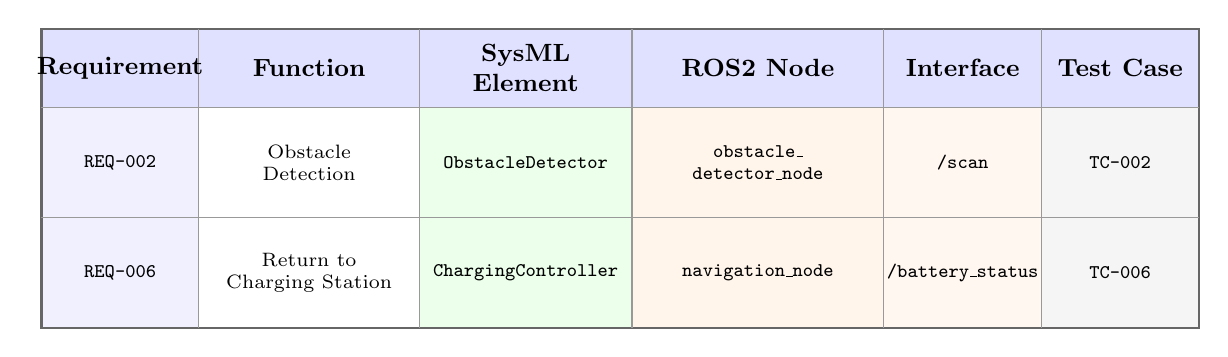
\begin{tikzpicture}[
    every node/.style={font=\small},
    x=1cm, y=1cm
]

% --- column boundaries (x) and row boundaries (y) in cm ---
% Columns: Requirement | Function | SysML system element | ROS2 node | Interface | Test case
% x0=0, x1=2.0, x2=4.8, x3=7.5, x4=10.7, x5=12.7, x6=14.7
% Rows (from top): y0=3.8 (header top), y1=2.8 (header bottom / row 1 top),
%                   y2=1.4 (row 1 bottom / row 2 top), y3=0 (row 2 bottom)

% --- column background for data rows (y3 to y1) ---
\fill[blue!6]   (0,0)    rectangle (2.0,2.8);
\fill[white]    (2.0,0)  rectangle (4.8,2.8);
\fill[green!8]  (4.8,0)  rectangle (7.5,2.8);
\fill[orange!8] (7.5,0)  rectangle (10.7,2.8);
\fill[orange!6] (10.7,0) rectangle (12.7,2.8);
\fill[black!4]  (12.7,0) rectangle (14.7,2.8);

% --- shade the header row on top ---
\fill[blue!12] (0,2.8) rectangle (14.7,3.8);

% --- grid lines: outer frame ---
\draw[black!60, thick] (0,0) rectangle (14.7,3.8);

% --- grid lines: vertical column separators ---
\draw[black!40] (2.0,0)  -- (2.0,3.8);
\draw[black!40] (4.8,0)  -- (4.8,3.8);
\draw[black!40] (7.5,0)  -- (7.5,3.8);
\draw[black!40] (10.7,0) -- (10.7,3.8);
\draw[black!40] (12.7,0) -- (12.7,3.8);

% --- grid lines: horizontal row separators ---
\draw[black!40] (0,1.4) -- (14.7,1.4);
\draw[black!40] (0,2.8) -- (14.7,2.8);

% --- header text ---
\node[font=\small\bfseries] at (1.0,3.3)  {Requirement};
\node[font=\small\bfseries] at (3.4,3.3)  {Function};
\node[font=\small\bfseries, align=center] at (6.15,3.3) {SysML\\Element};
\node[font=\small\bfseries] at (9.1,3.3)  {ROS2 Node};
\node[font=\small\bfseries] at (11.7,3.3) {Interface};
\node[font=\small\bfseries] at (13.7,3.3) {Test Case};

% --- row 1: REQ-002 ---
\node[font=\scriptsize] at (1.0,2.1)  {\texttt{REQ-002}};
\node[font=\scriptsize, align=center] at (3.4,2.1)  {Obstacle\\Detection};
\node[font=\scriptsize] at (6.15,2.1) {\texttt{ObstacleDetector}};
\node[font=\scriptsize, align=center] at (9.1,2.1)  {\texttt{obstacle\_}\\\texttt{detector\_node}};
\node[font=\scriptsize] at (11.7,2.1) {\texttt{/scan}};
\node[font=\scriptsize] at (13.7,2.1) {\texttt{TC-002}};

% --- row 2: REQ-006 ---
\node[font=\scriptsize] at (1.0,0.7)  {\texttt{REQ-006}};
\node[font=\scriptsize, align=center] at (3.4,0.7)  {Return to\\Charging Station};
\node[font=\scriptsize] at (6.15,0.7) {\texttt{ChargingController}};
\node[font=\scriptsize] at (9.1,0.7)  {\texttt{navigation\_node}};
\node[font=\scriptsize] at (11.7,0.7) {\texttt{/battery\_status}};
\node[font=\scriptsize] at (13.7,0.7) {\texttt{TC-006}};

\end{tikzpicture}


%     \caption{Excerpt from a traceability matrix: each row connects
%       a requirement, through a function, system element, and ROS2
%       node, to a test case.}
%     \label{fig:kap20-traceability-matrix}
%   \end{figure}
%
% Required packages (already loaded in main_en.tex): tikz
% Required TikZ libraries: positioning, arrows.meta, shadows, calc
% =====================================================================

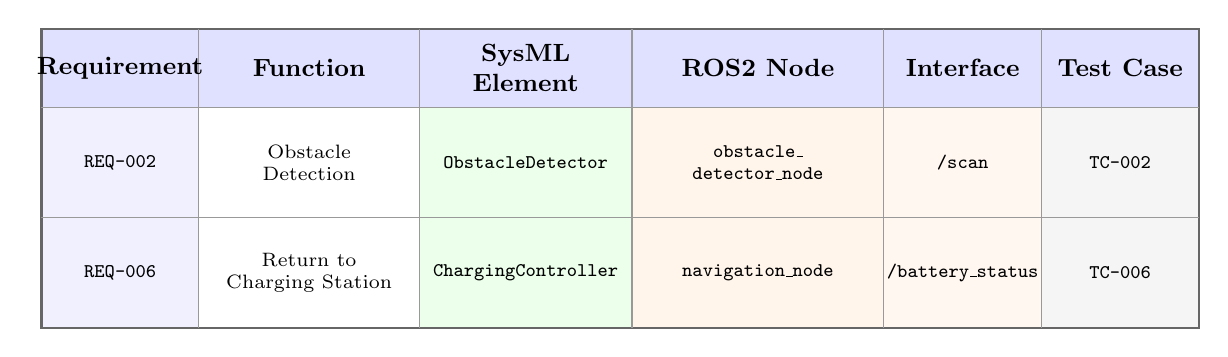
\begin{tikzpicture}[
    every node/.style={font=\small},
    x=1cm, y=1cm
]

% --- column boundaries (x) and row boundaries (y) in cm ---
% Columns: Requirement | Function | SysML system element | ROS2 node | Interface | Test case
% x0=0, x1=2.0, x2=4.8, x3=7.5, x4=10.7, x5=12.7, x6=14.7
% Rows (from top): y0=3.8 (header top), y1=2.8 (header bottom / row 1 top),
%                   y2=1.4 (row 1 bottom / row 2 top), y3=0 (row 2 bottom)

% --- column background for data rows (y3 to y1) ---
\fill[blue!6]   (0,0)    rectangle (2.0,2.8);
\fill[white]    (2.0,0)  rectangle (4.8,2.8);
\fill[green!8]  (4.8,0)  rectangle (7.5,2.8);
\fill[orange!8] (7.5,0)  rectangle (10.7,2.8);
\fill[orange!6] (10.7,0) rectangle (12.7,2.8);
\fill[black!4]  (12.7,0) rectangle (14.7,2.8);

% --- shade the header row on top ---
\fill[blue!12] (0,2.8) rectangle (14.7,3.8);

% --- grid lines: outer frame ---
\draw[black!60, thick] (0,0) rectangle (14.7,3.8);

% --- grid lines: vertical column separators ---
\draw[black!40] (2.0,0)  -- (2.0,3.8);
\draw[black!40] (4.8,0)  -- (4.8,3.8);
\draw[black!40] (7.5,0)  -- (7.5,3.8);
\draw[black!40] (10.7,0) -- (10.7,3.8);
\draw[black!40] (12.7,0) -- (12.7,3.8);

% --- grid lines: horizontal row separators ---
\draw[black!40] (0,1.4) -- (14.7,1.4);
\draw[black!40] (0,2.8) -- (14.7,2.8);

% --- header text ---
\node[font=\small\bfseries] at (1.0,3.3)  {Requirement};
\node[font=\small\bfseries] at (3.4,3.3)  {Function};
\node[font=\small\bfseries, align=center] at (6.15,3.3) {SysML\\Element};
\node[font=\small\bfseries] at (9.1,3.3)  {ROS2 Node};
\node[font=\small\bfseries] at (11.7,3.3) {Interface};
\node[font=\small\bfseries] at (13.7,3.3) {Test Case};

% --- row 1: REQ-002 ---
\node[font=\scriptsize] at (1.0,2.1)  {\texttt{REQ-002}};
\node[font=\scriptsize, align=center] at (3.4,2.1)  {Obstacle\\Detection};
\node[font=\scriptsize] at (6.15,2.1) {\texttt{ObstacleDetector}};
\node[font=\scriptsize, align=center] at (9.1,2.1)  {\texttt{obstacle\_}\\\texttt{detector\_node}};
\node[font=\scriptsize] at (11.7,2.1) {\texttt{/scan}};
\node[font=\scriptsize] at (13.7,2.1) {\texttt{TC-002}};

% --- row 2: REQ-006 ---
\node[font=\scriptsize] at (1.0,0.7)  {\texttt{REQ-006}};
\node[font=\scriptsize, align=center] at (3.4,0.7)  {Return to\\Charging Station};
\node[font=\scriptsize] at (6.15,0.7) {\texttt{ChargingController}};
\node[font=\scriptsize] at (9.1,0.7)  {\texttt{navigation\_node}};
\node[font=\scriptsize] at (11.7,0.7) {\texttt{/battery\_status}};
\node[font=\scriptsize] at (13.7,0.7) {\texttt{TC-006}};

\end{tikzpicture}


%     \caption{Excerpt from a traceability matrix: each row connects
%       a requirement, through a function, system element, and ROS2
%       node, to a test case.}
%     \label{fig:kap20-traceability-matrix}
%   \end{figure}
%
% Required packages (already loaded in main_en.tex): tikz
% Required TikZ libraries: positioning, arrows.meta, shadows, calc
% =====================================================================

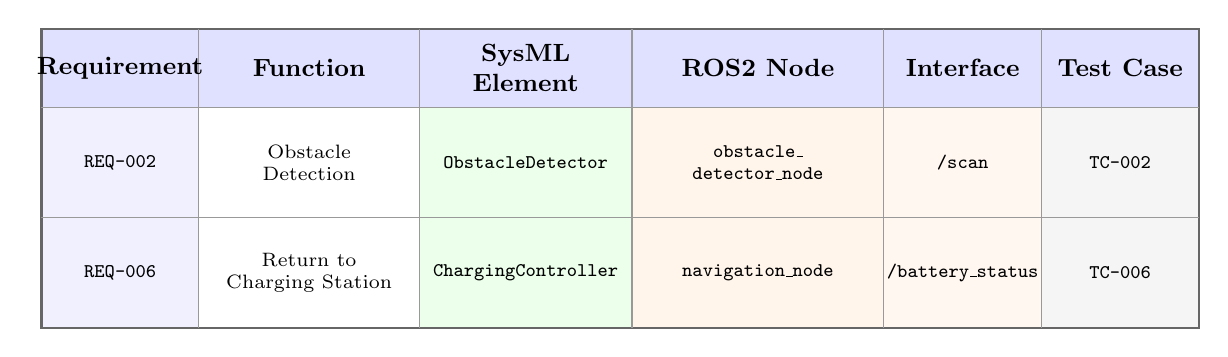
\begin{tikzpicture}[
    every node/.style={font=\small},
    x=1cm, y=1cm
]

% --- column boundaries (x) and row boundaries (y) in cm ---
% Columns: Requirement | Function | SysML system element | ROS2 node | Interface | Test case
% x0=0, x1=2.0, x2=4.8, x3=7.5, x4=10.7, x5=12.7, x6=14.7
% Rows (from top): y0=3.8 (header top), y1=2.8 (header bottom / row 1 top),
%                   y2=1.4 (row 1 bottom / row 2 top), y3=0 (row 2 bottom)

% --- column background for data rows (y3 to y1) ---
\fill[blue!6]   (0,0)    rectangle (2.0,2.8);
\fill[white]    (2.0,0)  rectangle (4.8,2.8);
\fill[green!8]  (4.8,0)  rectangle (7.5,2.8);
\fill[orange!8] (7.5,0)  rectangle (10.7,2.8);
\fill[orange!6] (10.7,0) rectangle (12.7,2.8);
\fill[black!4]  (12.7,0) rectangle (14.7,2.8);

% --- shade the header row on top ---
\fill[blue!12] (0,2.8) rectangle (14.7,3.8);

% --- grid lines: outer frame ---
\draw[black!60, thick] (0,0) rectangle (14.7,3.8);

% --- grid lines: vertical column separators ---
\draw[black!40] (2.0,0)  -- (2.0,3.8);
\draw[black!40] (4.8,0)  -- (4.8,3.8);
\draw[black!40] (7.5,0)  -- (7.5,3.8);
\draw[black!40] (10.7,0) -- (10.7,3.8);
\draw[black!40] (12.7,0) -- (12.7,3.8);

% --- grid lines: horizontal row separators ---
\draw[black!40] (0,1.4) -- (14.7,1.4);
\draw[black!40] (0,2.8) -- (14.7,2.8);

% --- header text ---
\node[font=\small\bfseries] at (1.0,3.3)  {Requirement};
\node[font=\small\bfseries] at (3.4,3.3)  {Function};
\node[font=\small\bfseries, align=center] at (6.15,3.3) {SysML\\Element};
\node[font=\small\bfseries] at (9.1,3.3)  {ROS2 Node};
\node[font=\small\bfseries] at (11.7,3.3) {Interface};
\node[font=\small\bfseries] at (13.7,3.3) {Test Case};

% --- row 1: REQ-002 ---
\node[font=\scriptsize] at (1.0,2.1)  {\texttt{REQ-002}};
\node[font=\scriptsize, align=center] at (3.4,2.1)  {Obstacle\\Detection};
\node[font=\scriptsize] at (6.15,2.1) {\texttt{ObstacleDetector}};
\node[font=\scriptsize, align=center] at (9.1,2.1)  {\texttt{obstacle\_}\\\texttt{detector\_node}};
\node[font=\scriptsize] at (11.7,2.1) {\texttt{/scan}};
\node[font=\scriptsize] at (13.7,2.1) {\texttt{TC-002}};

% --- row 2: REQ-006 ---
\node[font=\scriptsize] at (1.0,0.7)  {\texttt{REQ-006}};
\node[font=\scriptsize, align=center] at (3.4,0.7)  {Return to\\Charging Station};
\node[font=\scriptsize] at (6.15,0.7) {\texttt{ChargingController}};
\node[font=\scriptsize] at (9.1,0.7)  {\texttt{navigation\_node}};
\node[font=\scriptsize] at (11.7,0.7) {\texttt{/battery\_status}};
\node[font=\scriptsize] at (13.7,0.7) {\texttt{TC-006}};

\end{tikzpicture}

